
\section{Testes}

O teste do projeto foi organizado em pastas específicas de cada teste, localizadas na pasta \textit{/test} da raiz 
do projeto \textit{RCP-MO601-Project-01}. Cada pasta específica representa um teste no qual se especifica o circuito 
lógico desejado (\textit{circuito.hdl}), os estímulos (\textit{estimulos.txt}) a serem processados ao longo do tempo (valores de variáveis e/ou indicadores de tempo), 
os arquivos com as saídas esperadas (\textit{esperado0.csv e esperado1.csv}) e os arquivos resultadntes da simulação 
(\textit{saida0.csv e saida1.csv})

Novos testes podem ser adicionados à pasta principal de testes, contudo o simulador exige a
presença dos arquivos (\textit{circuito.hdl}), os estímulos (\textit{estimulos.txt}).

Durante a simulação dos testes, conforme pode-se observar no \textit{algorithm \space \ref{alg:simulacao}}, 
todas as pastas de testes específicos são consideradas, seus arquivos de entrada são 
processados e os resultados (saídas) são armazenados nas mesmas.

% \begin{figure}[H]
%     \centering
%     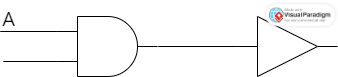
\includegraphics[scale=0.6]{Imagens/test_01_diagram.png}
%     \caption{Diagrama do circuito lógico test_01}
%     \label{fig:teste_01}
% \end{figure}

% \begin{figure}[H]
%     \centering
%     
\includegraphics[scale=0.6]{Imagens/LOGO-EQ.jpg}
%     \caption {Exemplo de figura}
%     \label{fig:logo}
% \end{figure}

% \begin{figure}[H]
%     \centering
%     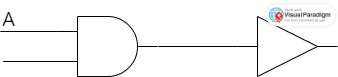
\includegraphics[scale=0.6]{Imagens/test_01_diagram.jpg}
%     \caption {Exemplo de figura}
%     \label{fig:logo2}
% \end{figure}

% Citando verge \cite{verge_ai_generator}